\documentclass[10pt]{report}

\usepackage[utf8]{inputenc} % Required for inputting international characters
\usepackage[T1]{fontenc} % Output font encoding for international characters
\usepackage[demo]{graphicx} % images % get rid of [demo] for black box removal
\usepackage{fancyhdr} % headers and footers
\usepackage{parskip} % paragraph
\usepackage{geometry} % shapes
\usepackage{hyperref} % Links
\usepackage{pdflscape} % making a page landscape
\usepackage{xcolor}
\usepackage[shortlabels]{enumitem}
\usepackage{multirow}

\graphicspath{{../images/}}

% margins and page size
\geometry{
a4paper,
left=30mm,
top=25mm,
right=30mm,
bottom=25mm
}

\begin{document}

\begin{titlepage}
\center
{\huge\bfseries Computer Graphics 

Aum Patel
}

\end{titlepage}
\tableofcontents
\chapter{Question 1 - Geometry and vertex attributes}

Y-axis up, X axis left to right and Z axis towards you is a Right handed coordinate system. I have proven this by using my right-hand with the X-axis being on the thumb, the Y-axis being on the first finger and the Z-axis being on my middle finger and rotating it to meet the 3 requirements. You cannot rotate the left hand to do this.

\begin{figure}[h]
    \centering
    \fbox{\includegraphics[width = 5cm ]{Right_Hand_Axis.png}}
    \caption{Image of hand with axis labeled.}
\end{figure}

I decided to draw out the model I was going to make in Blender first and then place the vertices on top of it. 

The colors of the axis are consistent in all images: \textcolor{red}{Red : X} , \textcolor{green}{Green : Y} , \textcolor{blue}{Blue : Z}

\begin{figure}[h]
    \centering
    \fbox{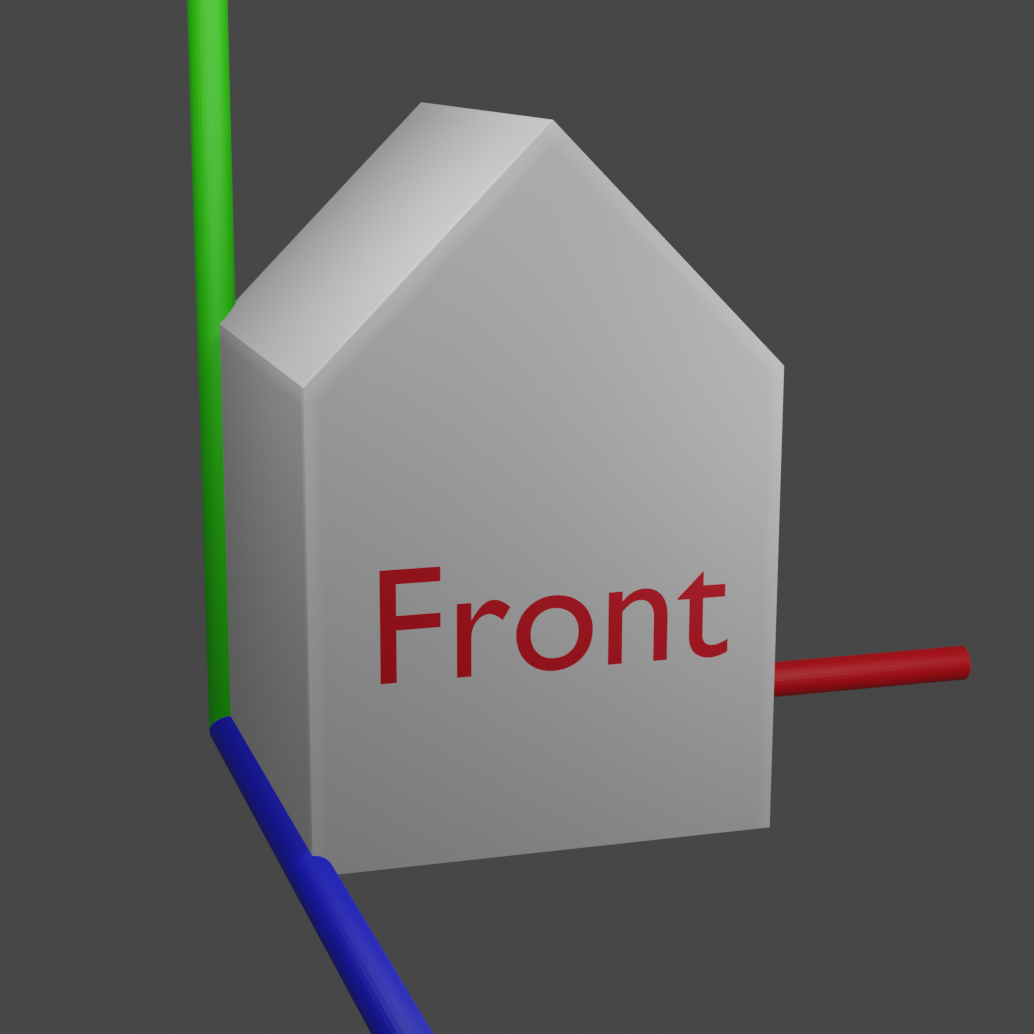
\includegraphics[width = 5cm ]{house_blender.png}}
    \caption{House in blender with drawn axis.}
\end{figure}

I chose the bottom vertex on the rear left of the house as the origin as I would only have to work with positive numbers for the rest of the vertices, and they would also be round numbers (except for the roof) as I am going to make the house with a square base of 1x1. 

Below is a wireframe view of the same house with the coordinates labeled.
\begin{figure}[h]
    \centering
    \fbox{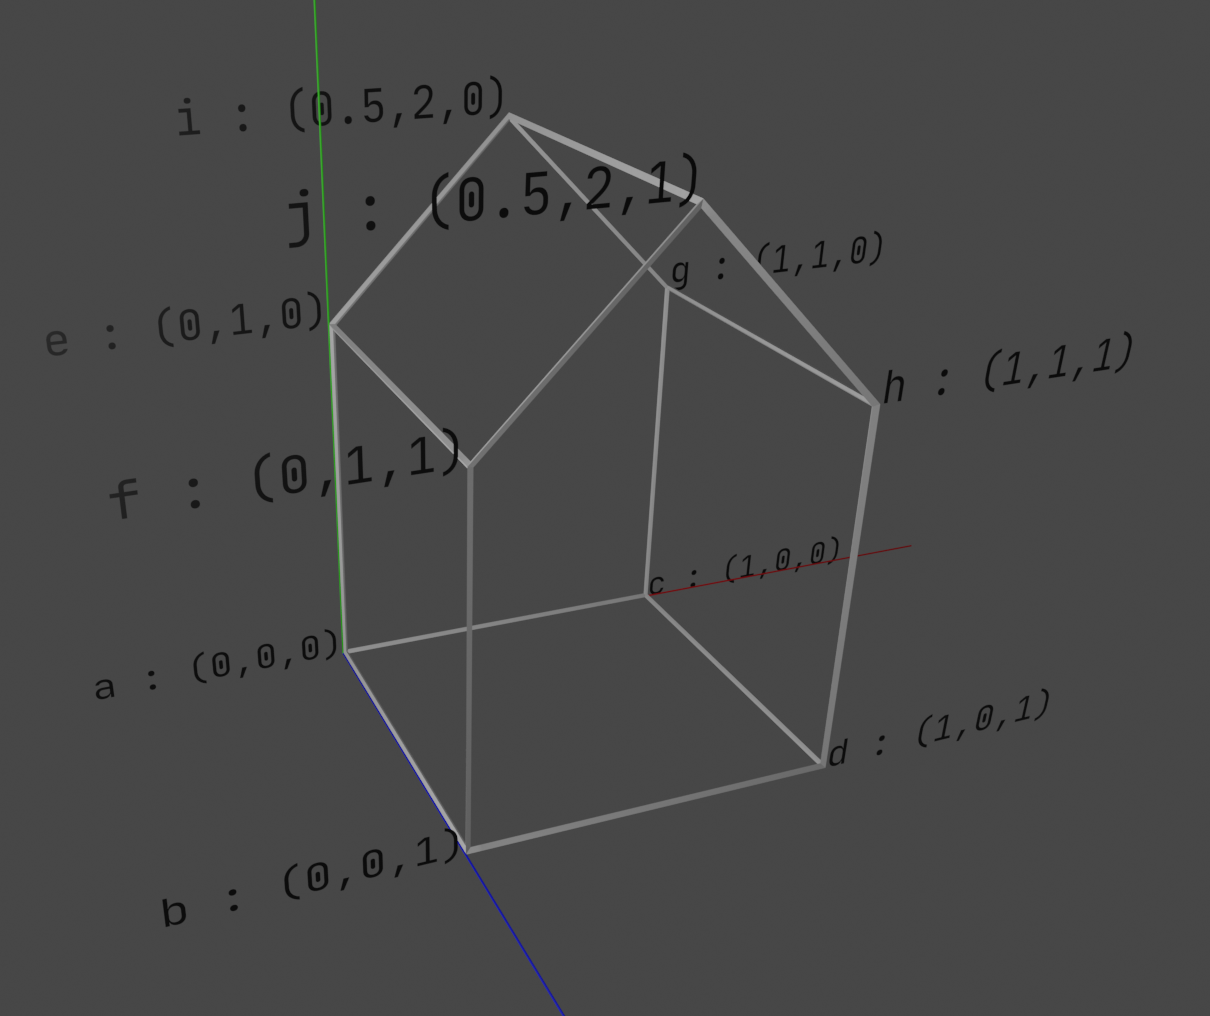
\includegraphics[width = 10cm ]{house_blender_wireframe_with_coord.png}}
    \caption{House in blender with wireframe and coordinates.}
\end{figure}

Coordinates for the vertices:
\begin{enumerate}[(a)]
    \item (0, 0, 0)
    \item (0, 0, 1)
    \item (1, 0, 0)
    \item (1, 0, 1)
    \item (0, 1, 0)
    \item (0, 1, 1)
    \item (1, 1, 0)
    \item (1, 1, 1)
    \item (0.5, 2, 0)
    \item (0.5, 2, 1)
\end{enumerate}

16 triangles will be used to make up the house, and there will be normals that are shared between them.

% Left
% (a, b, f)
% (a, f, e)

% Front
% (b, h, f)
% (b, d, h)
% (f, h, j)

% Right
% (d, g, h)
% (d, c, g)

% Back
% (c, e, g)
% (c, a, e)
% (g, e, i)

% Base
% (a, c, b)
% (b, c, d)

% Roof Left
% (e, j, i)
% (e, f, j)

% Roof Right
% (h, i, j)
% (h, g, i)



I calculated the vector normals by using the following equation:

If we have 3 vectors that make up a a triangle in an anti-clockwise manner: \(V0, V1, V2\), to calculate the normal facing outwards we do:

\(A = V1 - V0\)  |  \(B = V2 - V0\)

\(Normal = A \times B\)

Doing this with the first triangle on the table (triangle on the left face of the house) give you:

\(A = (0, 0, 1) - (0, 0, 0)\) \\ \(A = (0, 0, 1)\)

\(B = (0, 1, 1) - (0, 0, 0)\) \\ \(B = (0, 1, 1)\)

\(Normal = (0, 0, 1) \times (0, 1, 1)\) \\ \(Normal = (-1, 0, 0)\)

I confirmed this calculation to be correct by looking at the shape itself in 3D space, and \((-1, 0, 0)\) is the normal that would be correct.

I had no need to normalise the vectors as they output from the cross product was a sensible number.

Same calculation is done for the rest of the sides, triangles facing the same direction will have the same surface normals.

\begin{table}
    \begin{tabular}{|l|l|} 
    \hline
    \textbf{ Triangles } & \textbf{Normals }              \\ 
    \hline
    (a, b, f)            & \multirow{2}{*}{(-1, 0, 0)}    \\
    (a, f, e)            &                                \\ 
    \hline
    (b, h, f)            & \multirow{3}{*}{(0, 0, 1)}     \\
    (b, d, h)            &                                \\
    (f, h, j)            &                                \\ 
    \hline
    (d, g, h)            & \multirow{2}{*}{(1, 0, 0)}     \\
    (d, c, g)            &                                \\ 
    \hline
    (c, e, g)            & \multirow{3}{*}{(0, 0, -1)}    \\
    (c, a, e)            &                                \\
    (g, e, i)            &                                \\ 
    \hline
    (a, c, b)            & \multirow{2}{*}{(0, -1, 0)}    \\
    (b, c, d)            &                                \\ 
    \hline
    (e, j, i)            & \multirow{2}{*}{(-1, 0.5, 0)}  \\
    (e, f, j)            &                                \\ 
    \hline
    (h, i, j)            & \multirow{2}{*}{(1, 0.5, 0)}   \\
    (h, g, i)            &                                \\
    \hline
    \end{tabular}
\end{table}

\newpage

To write the .obj file, I have to change the alphabetical indices that I have been using into numerical. I have rounded the numbers to 6 decimal places. I have the same number of vertex normals as vertices as I decided to make the shape smooth shaded. 

NOTE THE VERTEX NORMALS HAVE NOT BEEN NORMALISED.


\begin{enumerate}[v]
    \item 0 0 0 % 1 a
    \item 0 0 1 % 2 b
    \item 1 0 0 % 3 c
    \item 1 0 1 % 4 d
    \item 0 1 0 % 5 e
    \item 0 1 1 % 6 f
    \item 1 1 0 % 7 g
    \item 1 1 1 % 8 h
    \item 0.5 2 0 % 9 i
    \item 0.5 2 1 % 10 j
\end{enumerate}     
% normalize vector (-0.333333333333, -0.333333333333, -0.333333333333)
% normalize vector (-0.333333333333, -0.333333333333, 0.333333333333)
% normalize vector (0.333333333333 ,-0.333333333333,-0.333333333333)
% normalize vector (0.333333333333 ,-0.333333333333,0.333333333333)
% normalize vector (-0.66666666667, 0.1666666667,-0.333333333333)
% normalize vector (-0.66666666667, 0.1666666667,0.333333333333)
% normalize vector (0.0, 0.1666666667, -0.333333333333)
% normalize vector (0.0, 0.1666666667, 0.333333333333)
% normalize vector (0.0, 0.333333333333, -0.333333333333)
% normalize vector (0.0, 0.333333333333, 0.333333333333)
\begin{enumerate}[vn]
    \item -0.333333 -0.333333 -0.333333 % 1 a
    \item -0.333333 -0.333333 0.333333 % 2 b
    \item 0.333333 -0.333333 -0.333333 % 3 c
    \item 0.333333 -0.333333 0.333333 % 4 d
    \item -0.666667 0.166667 -0.333333 % 5 e
    \item -0.666667 0.166667 0.333333 % 6 f
    \item 0.0 0.166667 -0.333333 % 7 g
    \item 0.0 0.166667 0.333333 % 8 h
    \item 0.0 0.333333 -0.333333 % 9 i
    \item 0.0 0.333333 0.333333 % 10 j
\end{enumerate}  
usemtl matWall
\begin{enumerate}[f]
    \item 1//1 2//2 6//6
    \item 1//1 6//6 5//5
    \item 2//2 8//8 6//6
    \item 2//2 4//4 8//8
    \item 6//6 8//8 10//10
    \item 4//4 7//7 8//8
    \item 4//4 3//3 7//7
    \item 3//3 5//5 7//7
    \item 3//3 1//1 5//5
    \item 7//7 5//5 9//9
    \item 1//1 3//3 2//2
    \item 2//2 3//3 4//4
\end{enumerate}
usemtl matRoof
\begin{enumerate}[f]
    \item 5//5 10//10 9//9
    \item 5//5 6//6 10//10
    \item 8//8 9//9 10//10
    \item 8//8 7//7 9//9
\end{enumerate}


\chapter{Question 2 - Vertex Buffer Object(VBO) design and transformations}
\begin{center}
\begin{verbatim}
You now have to design a VBO to contain the vertex attributes for your house. Choose a suitable layout for your VBO and list the calls to OpenGL from your client program required to transfer the VBO to the GPU. These should be native OpenGL commands. Do not assume that you have the helper classes from the template. Ensure that you give the correct values for the position and stride for each of the vertex attributes in VBO.

Your house is to be translated so it is centred at a new position on the ground plane, rotated by an angle that is not a multiple of 90º in such a way that the house remains correctly positioned on the ground and scaled to some multiple of its size. Choose your own rotation,translation and scale and provide the calls to glm using a glUtilmatrix stack that will achieve the desired transformation. Also provide the code to transfer this information to the GPU
\end{verbatim}
\end{center}

My single VBO will look like this:
\begin{verbatim}
x y z x y z x y z r g b r g b r g b
\end{verbatim}
which is the standard format, making the attributes tightly packed.

I will add the vertices for the triangles into an array of floats of size 9, three coordinates per triangle in the counter-clockwise order they should be drawn to render outside, for example the first triangle will look like this:
{0, 0, 0
0, 0, 1
0, 1, 1}

As the RGB values are in the VBO, I will initialise them as an array of size 9 as well.
{1, 1, 1,
1, 1, 1,
1, 1, 1}



\end{document}